\section{Problem Overview}
Authoring scientific articles with interactive visualisations is difficult
and time-consuming. We provide examples of text we would like to generate
and link to figures, mostly taken from the IPCC AR6 report, working group 1.

\paragraph*{Example: laying out assumptions for the text:} at the start of
the report in the Summary For Policymakers (SPM), the authors provide a
quick explanation of some common words used to describe probabilities,
which we show in \figref{good-text-mapping}.
\begin{figure}
   \begin{subfigure}{0.49\textwidth}
      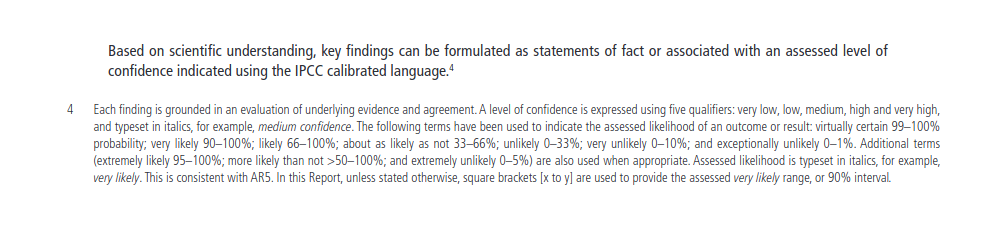
\includegraphics[width=\textwidth]{fig/ipcc-probabilities}
      \caption{Mapping probabilities onto text}
      \label{fig:good-text-mapping}
   \end{subfigure}
   \begin{subfigure}{0.49\textwidth}
      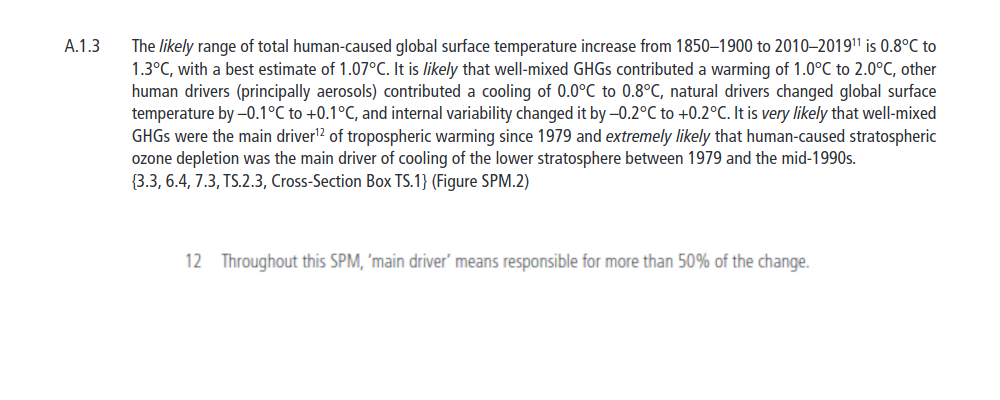
\includegraphics[width=\textwidth]{fig/ipcc-text-def-bad}
      \caption{Less helpful explanation of terminology}
      \label{fig:bad-text-mapping}
   \end{subfigure}
   \caption{Examples of good and bad mapping of numerical meaning onto text}
   \label{fig:text-mapping}
\end{figure}
We contrast this with the explanation given to the terminology ``main driver''
which the authors also believe merits an explanation, but the explanation they
give is not as helpful, pictured in \figref{bad-text-mapping}.

The explanation for the mapping of probabilities onto the text is simple,
and hopefully uncontroversial. The explanation contains all the information
required to understand what the use of a phrase of ``IPCC calibrated language''
means when it says ``X outcome is \textit{very likely}''. On the other hand,
the explanation of the meaning of ``main driver'' is poor, since it doesn't explain
what it means for something to ``be responsible for $50\%$ of the change''. 

\paragraph*{Synthesizing numerical/structural expressions related to data:}
\begin{figure}
      \begin{subfigure}{0.4\textwidth}
         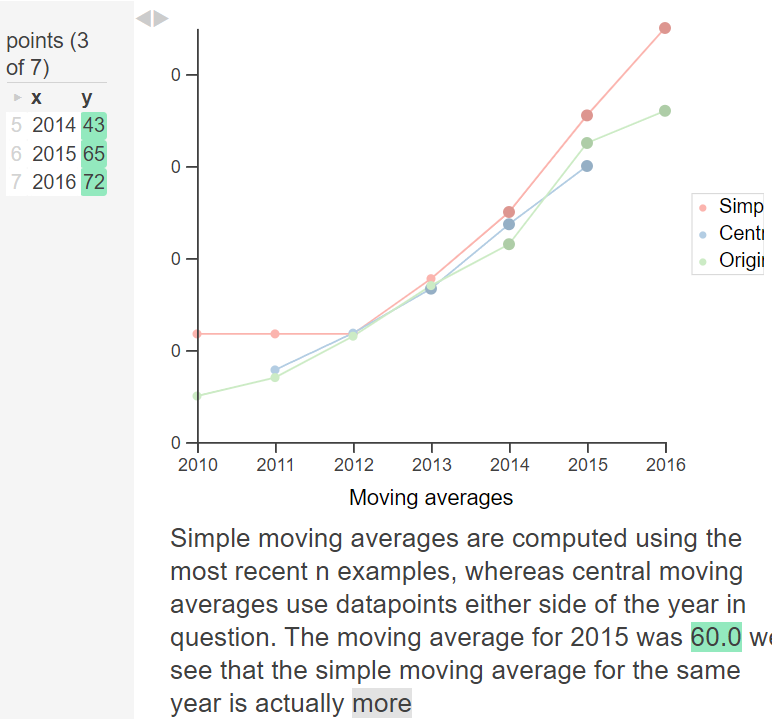
\includegraphics[width=\textwidth]{fig/text-viz.png}
         \caption{Example of text linking, using moving average example program}
         \label{fig:mavg}
      \end{subfigure}
      \hfill
      \begin{subfigure}{0.5\textwidth}
         \begin{subfigure}{\textwidth}
            \tiny
            \begin{lstlisting}[language=Fluid]
               ~\dots~
               "explain-1" :=
                  LinkedText( [ ~\dots~
                              , numToStr (getByX 2015 cavgs).y, " "
                              ~\dots~ ] )
               ~\dots~
            \end{lstlisting}
            \caption{Accessing data from chart points}
            \label{fig:synthex-1}
         \end{subfigure}
         \vfill
         \begin{subfigure}{\textwidth}
            \tiny
            \begin{lstlisting}[language=Fluid]
               ~\dots~
               let leqP n m = 
                  if n <= m
                  then "less"
                  else "more";
               ~\dots~
               , leqP (getByX 2015 savgs).y (getByX 2015 cavgs).y
               ~\dots~
            \end{lstlisting}
            \caption{generating text from results of data comparisons}
            \label{fig:synthex-2}
         \end{subfigure}
      \end{subfigure}
   \caption{Small Synthesis Examples}
   \label{fig:synthex}
\end{figure}
if we are referring to a simple aggregate summary of data, we want to be able
to synthesize an in-place expression that helps out explanation. For example,
if we are explaining a bar-chart, we might write code that looks like \figref{synthex-1}.

If we take a look at more realistic examples, we find something slightly different is
happening. Attached explanatory text tends to make reference to visual elements directly
-- for example referring to a chart rather than some data used in the charts creation --
and so we will need our solution to be able to handle structurally walking through values
when synthesizing code that references them. In \figref{structural-mappings}, the black
arrows show simple examples of the type of text that should be automatically linked to
the constructor of the visual element to which it refers. At this level, it refers to
\textit{graphs} (in our world: views) and \textit{panels} (in our world multiviews?).


\begin{figure}
   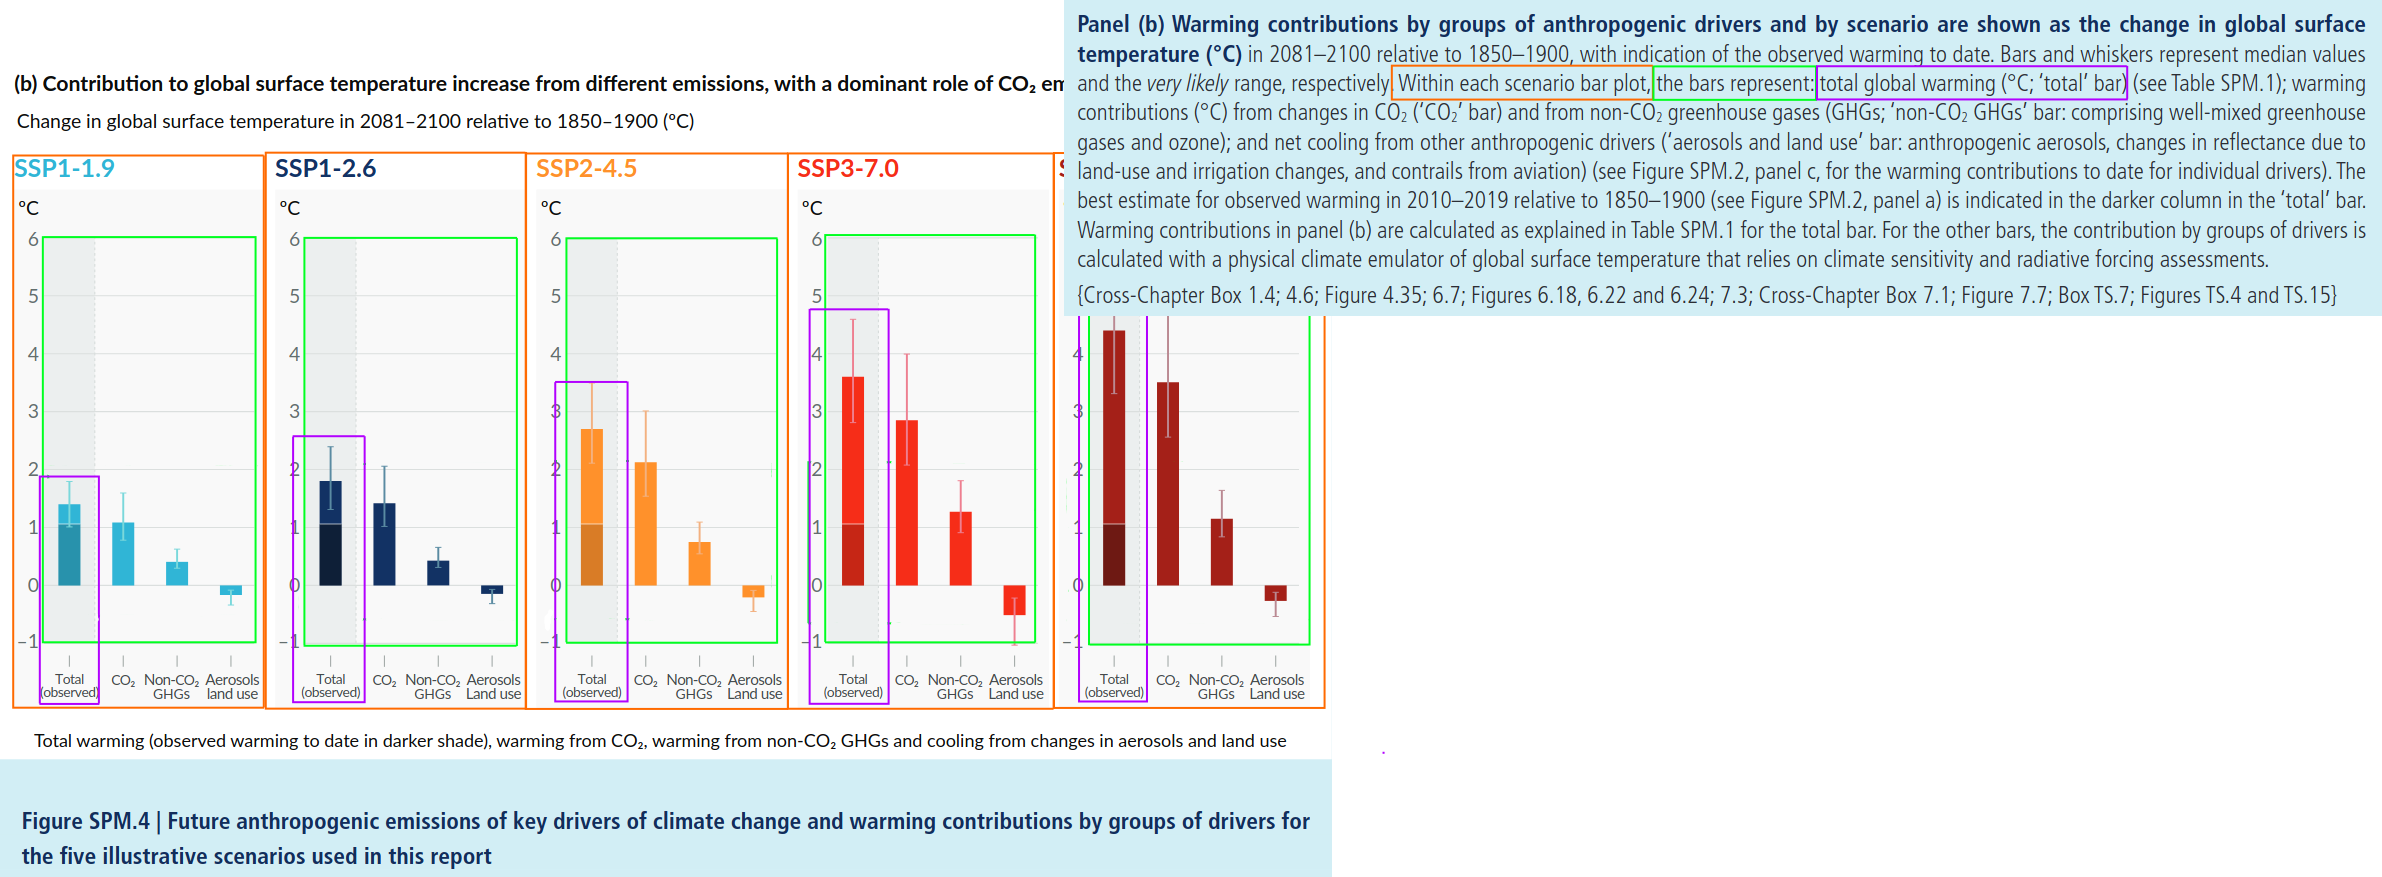
\includegraphics[width=\textwidth]{fig/ipcc-visual-elements.png}
   \caption{Examples of mapping text directly onto visual elements}
   \label{fig:structural-mappings}
\end{figure}
\paragraph*{Synthesizing string expressions based on those numerical expressions:}
this is similar to the nombre library in R, once we are able to synthesize references
to numerical expressions and data, we want to be able to take those, and use them to
create small strings to splice into an explanation. For example, in \figref{synthex-2}
we would like the tool to be able to synthesize both the function \kw{leqP}, and
the expression in situ, which then generates the last word in the caption appearing in
\figref{mavg}.
